\documentclass[11pt, openany, oneside, article, a4paper, twocolumn]{memoir}
\usepackage{lipsum}
\usepackage{fontspec}
\usepackage{csquotes}
\usepackage[backend=biber, style=phys, hyperref, url=false, sorting=none]{biblatex}
\usepackage{hyperref}

\addbibresource{references.bib}
%\setmainfont[
  %BoldFont={Chronicle Text G1 Bold},
  %ItalicFont={Chronicle Text G1 Italic},
  %BoldItalicFont={Chronicle Text G1 Bold Italic}
%]{Chronicle Text G1 Roman}
%\setmainfont[
  %BoldFont={Miller Text Bold},
  %ItalicFont={Miller Text Italic}
%]{Miller Text}

\setmainfont[
  BoldFont={Minion Pro Bold},
  ItalicFont={Minion Pro Italic},
  BoldItalicFont={Minion Pro Bold Italic}
]{Minion Pro}
\setsansfont[]{Consolas}

\setlength{\absleftindent}{5em}
\setlength{\absrightindent}{5em}
\renewcommand{\abstracttextfont}{\footnotesize}
\setlength{\columnsep}{24pt}
\setlength{\parskip}{0pt}
\newlength{\postabstractskip}
\setlength{\postabstractskip}{15pt}
\urlstyle{rm}

% \setbeforesecskip{2.5ex plus 1ex minus .2ex}
% \setaftersecskip{2.5ex plus 1ex minus .2ex}

%\newfontfamily\headingfont[
  %ItalicFont={Chronicle Display Italic},
%]{Chronicle Display}
%\newfontfamily\subheadingfont[]{Chronicle Display Light}

\begin{document}
\renewcommand{\thesection}{\Roman{section}.}
\renewcommand{\abstractname}{}
\renewcommand{\absnamepos}{empty}
\pretitle{\begin{center}\begingroup\fontsize{32pt}{28pt}\selectfont}
\posttitle{\par\endgroup\end{center}\vskip 0.5em}
%\renewcommand{\booktitlefont}{\small\headingfont}

\title{hoi ik ben een titel}
\author{Geert Kapteijns\thanks{\href{mailto:ghkapteijns@gmail.com}{ghkapteijns@gmail.com}}}
\date{\today}

\twocolumn[
  \maketitle
  \vspace{-15pt}
  \begin{onecolabstract}

    \noindent Universal free online access of scientific journal articles is
    within reach if universities and funders mandate their authors to
    self-archive their refereed manuscripts in an institutional archive (IR),
    upon acceptance in the (subscription) journals of their choice. This form
    of open access (OA), known as \emph{Green}, can be implemented unilaterally by the
    universities and funders at little cost. It should not be confused with
    \emph{Gold} OA, meaning OA through \emph{publishing} directly in an OA
    journal.

    I claim that the Dutch government and the association of universities
    (VSNU), by focussing on Gold prematurely, have made deals that will
    needlessly slow down the provision of access and maintain or even increase
    the publishers' profit margins. Sustainable Gold access (including
    copyright reform) will follow once universal Green has been reached and
    publishers only provide the organisation of peer-review and luxury services
    like enhanced PDFs or paper versions.

    Grassroots publishing initiatives, such as SciPost, politicize the
    community by offering a glimpse of a possible future. But if they are
    serious about subverting the publishing industry, they should, in addition to
    their innovative activities, put their full weight behind the optimal Green
    mandate.
  \end{onecolabstract}
  \vspace{\postabstractskip}
]

\saythanks

\section{Introduction}

The current accessibility of research journal articles is decidedly
suboptimal. Journal prices have been rising at 2.5 times the rate of
inflation the last couple of decades \cite{monograph_serial_costs,
suber2008open}, but even if all 28000 existing journals could be
subscribed to at production cost, universities would not be able to afford
them all \cite{harnad2008access}. This means that all researchers, even at
the richest institutions, do not have full access to the output of their
colleagues, and all researchers are denied the full impact of their
research, since they cannot reach the entirety of their intended audience.

It is unbearable that this \emph{access/impact problem} still persists,
because with the advent of the Web, articles can be reproduced and spread
at virtually no cost. Doubly unbearable, since the whole enterprise is
funded with tax-payer money for the benefit of society. 

The solution to the problem is, according to Stevan Harnad, closer to
raincoat science than rocket science. In a haiku \cite{harnad_raincoat}:

\blockquote{%
It's the online age\\
You're losing research impact\dots \\
Make it free online}

\begin{figure}
  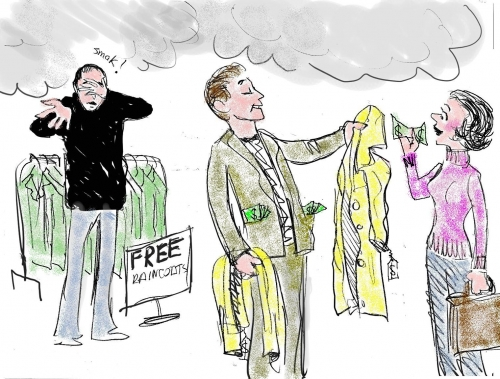
\includegraphics[width=\columnwidth]{rain4.jpg}
  \caption{Raincoat science by Judith Economos}
\end{figure}

In other words, authors can continue publishing in subscription journals,
but should as an extra adminstrative step \emph{publicly self-archive}
their refereed manuscripts. This practice, which Harnad has been
advocating since 1994 \cite{harnad1995subversive}, was laid out by the
Budapest Open Access Initiative (BOAI) as the first strategy to be
implemented \cite{boai}. It later came to be known as the \emph{Green}
strategy \cite{harnad2004access}. If it is universally adopted, the
access/impact problem would be solved.

Apart from public self-archiving (the \enquote{Green} road), the BOAI
described a complimentary \emph{Gold} strategy, namely to start a new
generation of journals that provide open access to the material they
publish. It is this second strategy that often has been misunderstood to
be the \emph{only} viable strategy of providing open access, by
scientists, media and politicians alike.

This is very unfortunate, since the Green solution is by far the most
cost-effective way of providing access \cite{houghton2013planting}
(10\%-20\% of what it presently costs to pay for Gold), can be decided on
by universities and funders unilaterally, without having to convince
publishers to alter their business model, and does not limit authors'
choices of journals in which they wish to publish.

Furthermore, it is plausible that once universal Green open access has been
achieved, existing subscription journals will face significant cancellation
pressure, because all their content is already available as self-archived
manuscripts. Those journals would be forced to cut costs and change their
business model, since the services they provide have been reduced to organizing
peer-review and providing enhanced PDFs and paper versions of the articles.
Thus, Green OA may leverage the transition to universal Gold
\cite{harnad2007green_road}.

In the rest of this article, I will first outline what is currently
understood to be the optimal Green open access policy. Then, I will show
that official policy in The Netherlands seriously deviates from this
consensus, needlessly slowing down the provision of access and maintaining
or even increasing the publishers' profit margins. Finally, I describe
that, since change is most likely to come from below, it is of vital
importance to the community that grassroots initiatives embrace the Green
mandate.

\section{The optimal Green mandate}

Apart from being beneficial to the community, self-archiving is also
advantageous for researchers personally due to increased uptake and
citation impact of their work \cite{gargouri2010self}. Yet, the majority
of scientists do not self-archive voluntarily. 62\% of journals endorse
self-archiving immediately and an additional 17\% endorse self-archiving
after an embargo period of six months or a year \cite{bjork2014anatomy}.
But estimates for the actual percentage of articles that is accessible in
this way (be it from an institutional archive, a preprint server or the
author's homepage) are far lower. The authors of \cite{bjork2010open} find
that in 2009 20\% of all journal articles were openly accessible, of which
12\% through self-archiving. In a subsequent study, the same authors find
an unchanged 12\% Green in 2014 \cite{bjork2014anatomy}. The authors of
\cite{khabsa2014number} find 24\% total OA (Green and Gold) in 2013. The
study in \cite{archambault2013tipping} is an outlier, finding 48\% total
OA, of which 34\% Green\footnote{The authors also include articles
published in \emph{hybrid} journals -- meaning subscription journals that
offer the option of providing open access for an additional author fee --
in this percentage, so the fraction of Green articles is presumably
slightly lower.}, already in 2008.

These numbers include unrefereed preprint versions (about 15\% in
\cite{bjork2014anatomy}), since the archived and published versions are
mostly matched by automated title/author/abstract matching. Furthermore,
archived manuscripts are scattered throughout the Web
\cite{kim2010faculty}, and archived versions that became available only
after a (possibly long) embargo period are counted.

In the domain of Physics and Astronomy, where sharing preprints has
historically played an important role \cite{brown2001evolution},
self-archiving is universally endorsed by publishers\footnote{This is an
example of \enquote{proof by intimidation.} Feel free to prove me wrong
using \cite{sherpa_romeo}. In any case, physicists, along with computer
scientists and mathematicians, have always freely shared their preprints
and refereed manuscripts. E-mail and later preprint servers became natural
tools to make this practice easier and were freely used, even before the
issue of self-archivation ended up in publisher contracts
\cite{brown2001evolution}. Publishers have, to the best of my knowledge,
never ordered anyone to take down a manuscript in these fields.}. The
preprint server arXiv, established in 1991, has become the canonical place
to share manuscripts. But even in this field, self-archiving is not
systematic, although the numbers are slightly higher. Estimates are that
around 20\% of papers that appear in Web of Science journals can be found
on arXiv, possibly as an unrefereed (preprint) version
\cite{bjork2010open, lariviere2014arxiv}. Some subfields, such as
astronomy and high-energy physics, have around 70\% Green, with the
percentage in top journals approaching 100\% \cite{gentil2010citinghep}.

If the benefits are clear, why do scientists refuse to self-archive?
Harnad lists many possible reasons \cite{harnad2006opening}, the most
prevalent being that (i) scientists think it is illegal, (ii) that it
causes their papers to be less likely to be accepted, and (iii) that
scientists are simply too lazy.

The solution is for universities and funders to \emph{mandate} their
researchers to self-archive. It is worth quoting Harnad's implementation proposal in full \cite{harnad2015openwhat}:

\begin{small}
\begin{enumerate}[(1)]
\item All research funding agency OA Mandates need to specify clearly and explicitly that the deposit of each
article must be in the author’s institutional repository (so the universities
and research institutions can monitor their own output and ensure compliance as
well as adopt mandates of their own for their unfunded research output).

\item All mandates should specify that the deposit (of the authors refereed, revised,
accepted final draft) must be done immediately upon acceptance for publication
(not on the date of publication, which is often much later, variable, not known
to the author, and frequently does not even correspond to the journal issue’s
published date of publication, if there is one).

\item All mandates should urge
(but not require) authors to make their immediate-deposit immediately-OA.
\item All mandates should urge (but not require) authors to reserve the right to make
their papers immediately-OA (and other re-use rights) in their contracts with
their publishers (as in the Harvard-style mandates).
\item All mandates should
shorten (or, better, not even mention) allowable OA embargoes (so as not to
encourage publishers to adopt them).
\item All repositories should implement the
automated "email eprint request" Button (for embargoed [non-OA] deposits).
\item All mandates should designate repository deposit as the sole mechanism for
submitting publications for performance review, research assessment, grant
application, or grant renewal.
\item All repositories should implement rich usage
and citation metrics in the institutional repositories as incentive for
compliance.
\end{enumerate}
\end{small}




\begin{itemize}
  \item estimating OA mandate effectiveness: MELIBEA score \cite{vincent2016estimating}
  \item fair use button \cite{sale2010open}
\end{itemize}

\section{Current institution and funder mandates in The Netherlands}

lorem

\section{Grassroots initiatives}

lorem

\printbibliography

%\twocolumn[
   %\begin{@twocolumnfalse}
     %\printbibliography
   %\end{@twocolumnfalse}
%]

\end{document}
